% Copyright 2021 Joel Feldman, Andrew Rechnitzer and Elyse Yeager, except where noted.
% This work is licensed under a Creative Commons Attribution-NonCommercial-ShareAlike 4.0 International License.
% https://creativecommons.org/licenses/by-nc-sa/4.0/


\begin{frame}{Table of Contents}
\mapofcontentsC{\cc}
\end{frame}
\section*{3.3: Exponential Growth and Decay}
%----------------------------------------------------------------------------------------
%----------------------------------------------------------------------------------------
%----------------------------------------------------------------------------------------
%----------------------------------------------------------------------------------------
\begin{frame}[t]{Radioactive Decay}
\note<1>{This is a first look at DEs. Take some time to point out how this equation looks different from what we're used to writing.}
The number of atoms in a sample that decay in a given time interval is proportional to the number of atoms in the sample.
\pause
\begin{block}{Differential Equation}
Let $Q=Q(t)$ be the amount of a radioactive substance at time $t$. Then for some positive constant $k$:
\[\frac{dQ}{dt} = -kQ\]
\end{block}\pause
\begin{block}{Solution -- Theorem~\eref{text}{thm:growthDEsoln}}
Let $\boxed{Q(t)=Ce^{-kt}}$, where $k$ and $C$ are constants. Then:\pause
\answer{\[\alert{\frac{dQ}{dt}(t)}=C\cdot e^{{-kt}} \cdot (-k)=-kCe^{-kt}=\alert{-kQ(t)}\]}
\end{block}
\note<3>{emphasize we're looking for a function that makes the DE true, not just a number}

\unote{Equation~\eref{text}{eq:carbonDating}}
\end{frame}
%----------------------------------------------------------------------------------------

%----------------------------------------------------------------------------------------
\begin{frame}[t]{Radioactive Decay}
\AnswerSpace
\only<2,4>{\AnswerYes}
\only<2>{\QuestionBar{1}{4}}
\only<3>{\AnswerBar{1}{4}}
\only<4>{\QuestionBar{2}{4}}
\only<5>{\AnswerBar{2}{4}}
\begin{block}{Quantity of a Radioactive Isotope}
\[Q(t)=Ce^{-kt}\]
$Q(t)$: quantity at time $t$
\end{block}
\vfill\pause
\begin{multicols}{2}
What is the sign of $Q(t)$?
\begin{itemize}
\alert<3-|handout:0>{\item[A.] positive or zero}
\item[B.] negative or zero
\item[C.] could be either
\item[D.] I don't know
\end{itemize}
\pause\pause\vfill
What is the sign of $C$?
\begin{itemize}
\alert<5-|handout:0>{\item[A.] positive or zero}
\item[B.] negative or zero
\item[C.] could be either
\item[D.] I don't know
\end{itemize}
\end{multicols}
\end{frame}
%----------------------------------------------------------------------------------------
\begin{frame}[t]
\begin{block}{Seaborgium Decay}
The amount of $^{266}Sg$ (Seaborgium-266) in a sample at time $t$ (measured in seconds) is given by
\[Q(t)=Ce^{-kt}\]
Let's approximate the half life of $^{266}Sg$ as 30 seconds. That is, every 30 seconds, the size of the sample halves.
\end{block}
 What are $C$ and $k$?
\AnswerYes\MoreSpace\QuestionBar{3}{4}
\unote{Example~\eref{text}{eg:carbonDatingHalfLife}}
\end{frame}
%----------------------------------------------------------------------------------------
\begin{frame}<handout:0>[t]
\AnswerSpace \only<1>{\AnswerYes\QuestionBar{3}{4}}
\only<2>{\AnswerBar{3}{4}} 
\[Q(t)=Ce^{-kt}\]
Every 30 seconds, the size of the sample halves. What are $C$ and $k$?\vfill\pause
\answer{
\begin{itemize}\color{answercolor}
\item[(1)] $Q(0)$ is the amount of $^{266}Sg$ at time 0: usually, the initial sample size.

\textcolor{M4}{$C$ is the quantity at time 0}
\item[(2)]The half-life of $^{266}Sg$ is 30 seconds.
So, if we're measuring $t$ in seconds, $Q(30)=\frac{1}{2}Q(0)$. 
\[\frac{1}{2}C=\frac{1}{2}Q(0)=Q(30)=Ce^{-30k}\]
\textcolor{M4}{$k=\dfrac{\log 2}{30}$}
\end{itemize}}
\unote{Example~\eref{text}{eg:carbonDatingHalfLife}}
\end{frame}
%----------------------------------------------------------------------------------------
\begin{frame}[t]
\unote{Example~\eref{text}{eg_3_3_1}}
\only<1>{\AnswerYes
\QuestionBar{4}{4}
A sample of radioactive matter is stored in a lab in 2000. In the year 2002, it is tested and found to contain 10 units of a particular radioactive isotope. In the year 2005, it is tested and found to contain only 2 units of that same isotope. How many units of the isotope were present in the year 2000?\vfill}
\only<2|handout:0>{\color{answercolor}
The quantity of the isotope $t$ years after 2000 is given by
\[Q(t)=Ce^{-kt}\]
where $C=Q(0)$ is the amount in the initial sample. Then the question asks us to solve for $C$, given
\[10=Q(2)=Ce^{-2k}\quad\mbox{and}\quad 2=Q(5)=Ce^{-5k}\]

Then
\[C=10e^{2k}=2e^{5k}\]
\[e^{3k}=5 \quad\implies\quad e^k=\sqrt[3]{5}\]
\[C=10e^{2k}=10\big(\sqrt[3]{5}\big)^2\approx 29\]}
\end{frame}
%----------------------------------------------------------------------------------------
%----------------------------------------------------------------

%----------------------------------------------------------------------------------------
\begin{frame}[t]{$Q'(t)=kQ(t)$}
\note<1>{Note the broader applicability of these equations }
\textcolor{C1}{The number of atoms in a sample that decay in a given time interval is proportional to the number of atoms in the sample.}
\pause\vfill

\textcolor{C3}{The rate of growth of a population in a given time interval is propotional to the number of individuals in the population, when the population has ample resources.}\pause\vfill

\textcolor{C4}{The amount of interest a bank account accrues in a given time interval is proportional to the balance in that bank account.}\vfill
\end{frame}
%----------------------------------------------------------------

%----------------------------------------------------------------------------------------
\begin{frame}[t]
\AnswerSpace
\only<2-3>{\AnswerYes}\only<2>{\MoreSpace}
\only<3>{\QuestionBar{1}{3}}\only<4->{\AnswerBar{1}{3}}
\only<1-2>{
\begin{block}{Exponential Growth -- Theorem~\eref{text}{thm:growthDEsoln}}
Let $Q=Q(t)$ satisfy:
\[\frac{dQ}{dt} = kQ\] for some constant $k$. Then for some constant $C=Q(0)$,
\[Q(t)=Ce^{kt}\] 
\end{block}}\pause
 Suppose $y(t)$ is a function with the properties that
\[\frac{dy}{dt}+3y=0 \quad\mbox{and}\quad y(1)=2.\]
What is $y(t)$? \pause\pause\vfill
\color{answercolor}
\answer{$\diff{y}{t}=-3y$, so $y(t)=Ce^{-3t}$ by the result above. 

\medskip
To solve for $C$, we set $t=1$:
\[2=y(1)=Ce^{-3}\implies C=2e^3\]
So,
\[y(t)=2{e^3}\cdot e^{-3t}=2e^{3(1-t)}\]}
\end{frame}
%----------------------------------------------------------------------------------------
\begin{frame}[t]{Population Growth}
\AnswerSpace\only<1>{\AnswerYes\QuestionBar{2}{3}}
\only<2>{\AnswerBar{2}{3}}
Suppose   a petri dish starts with a culture of 100 bacteria cells and a limited amount of food and space. The population of the culture at different times is given in the table below. At approximately what time did the culture start to show signs of limited resources?
\begin{multicols}{2}
\begin{tabular}{c|r}
time & population\\
\hline
0&100\\
1&1000\\
3&100000\\
5&1000000\\
\end{tabular}
\vfill\pause
\answer{\color{answercolor}
\small All the populations before $t=5$ follow $B(t)=100\cdot 10^t
=100e^{t\log 10 }$. At $t=5$ they do not; so some time between $t=3$ and $t=5$, the bacteria started reproducing at a slower rate.

}
\end{multicols}
\end{frame}
%----------------------------------------------------------------------------------------
%----------------------------------------------------------------------------------------
\begin{frame}[t]{Flu Season}
\only<1>{
\QuestionBar{3}{3}\AnswerYes
The CDC keeps records (\href{http://gis.cdc.gov/grasp/fluview/fluportaldashboard.html}{link}) on the number of flu cases in the US by week. At the start of the flu season, the 40th week of 2014, there are 100 cases of a particular strain. Five weeks later (at week 45), there are 506 cases. What do you think  was the first week to have 5,000 cases? What about 10,000 cases?}
\only<2|handout:0>{ 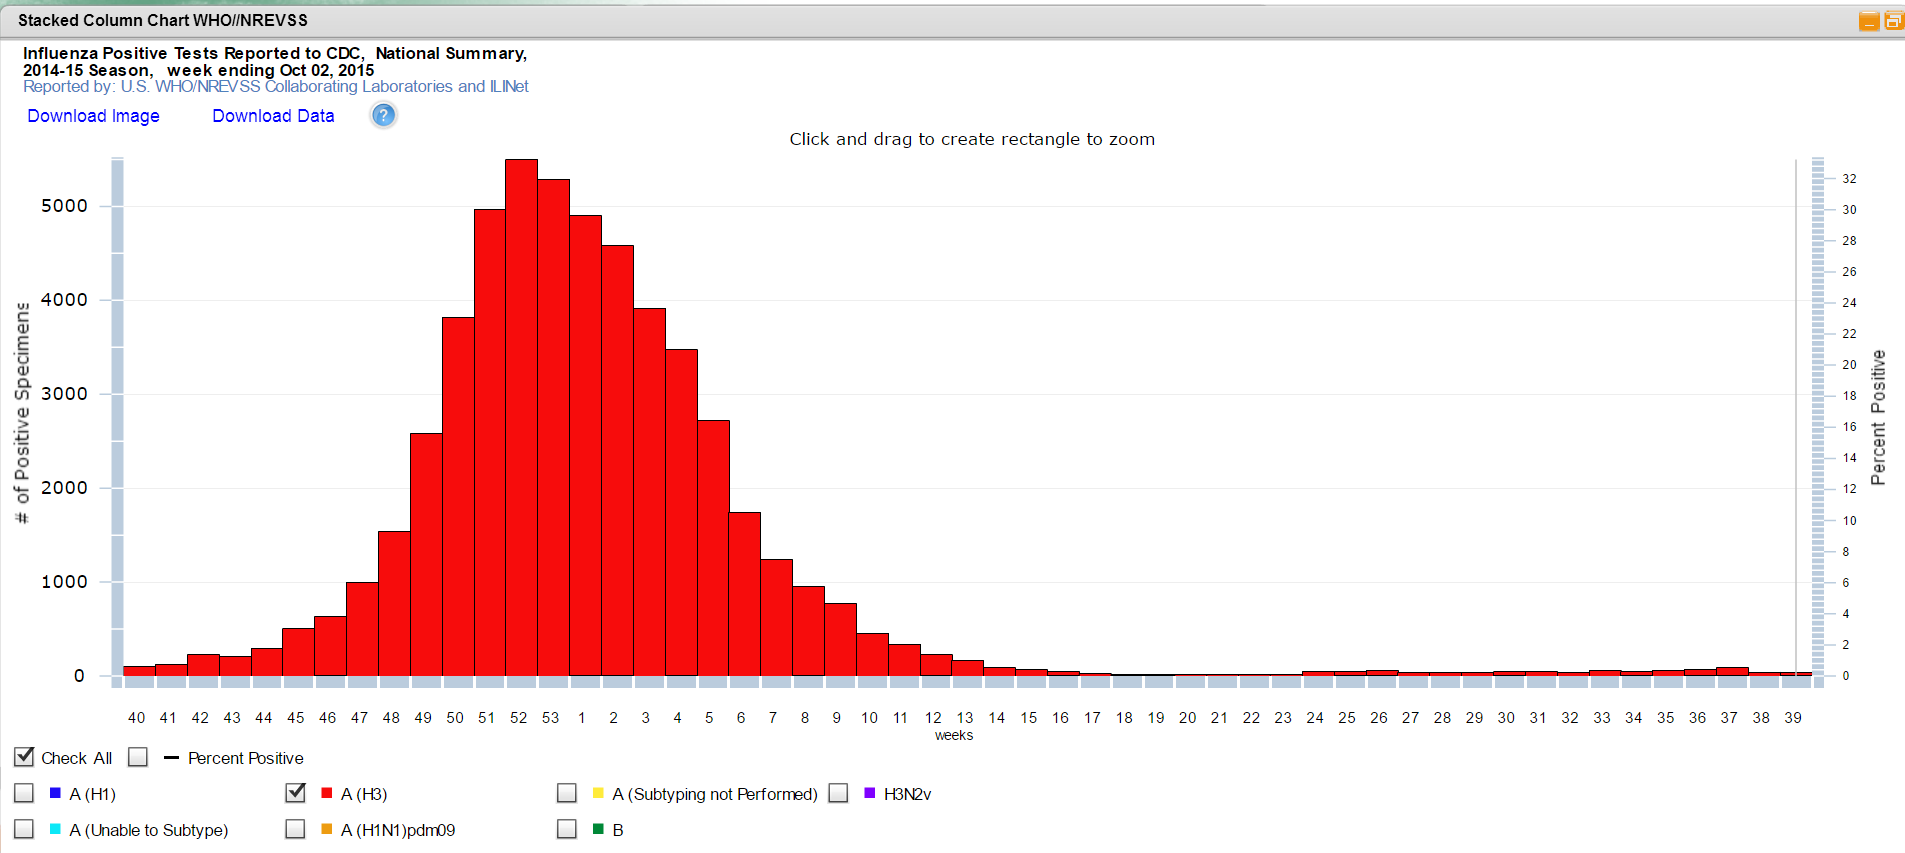
\includegraphics[height=0.9\textheight]{fig/H3}}
%\only<3|handout:0>{\AnswerBar{3}{3} 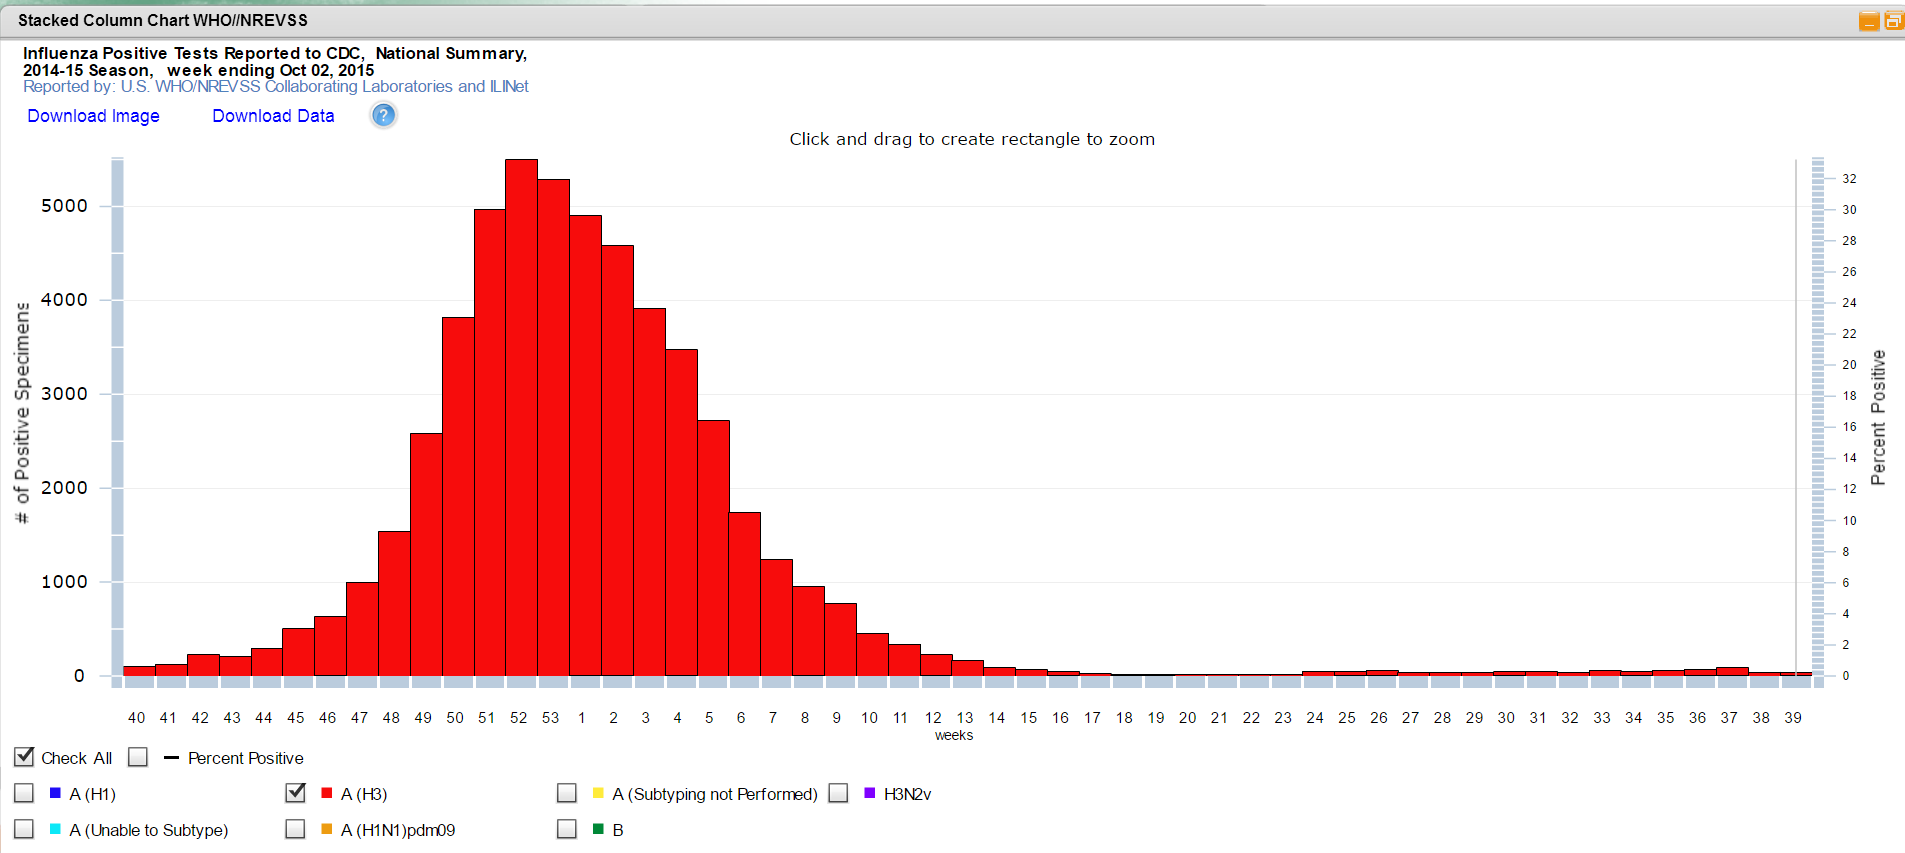
\includegraphics[width=\framewidth]{fig/H3}}
\only<2>{
 \index{ 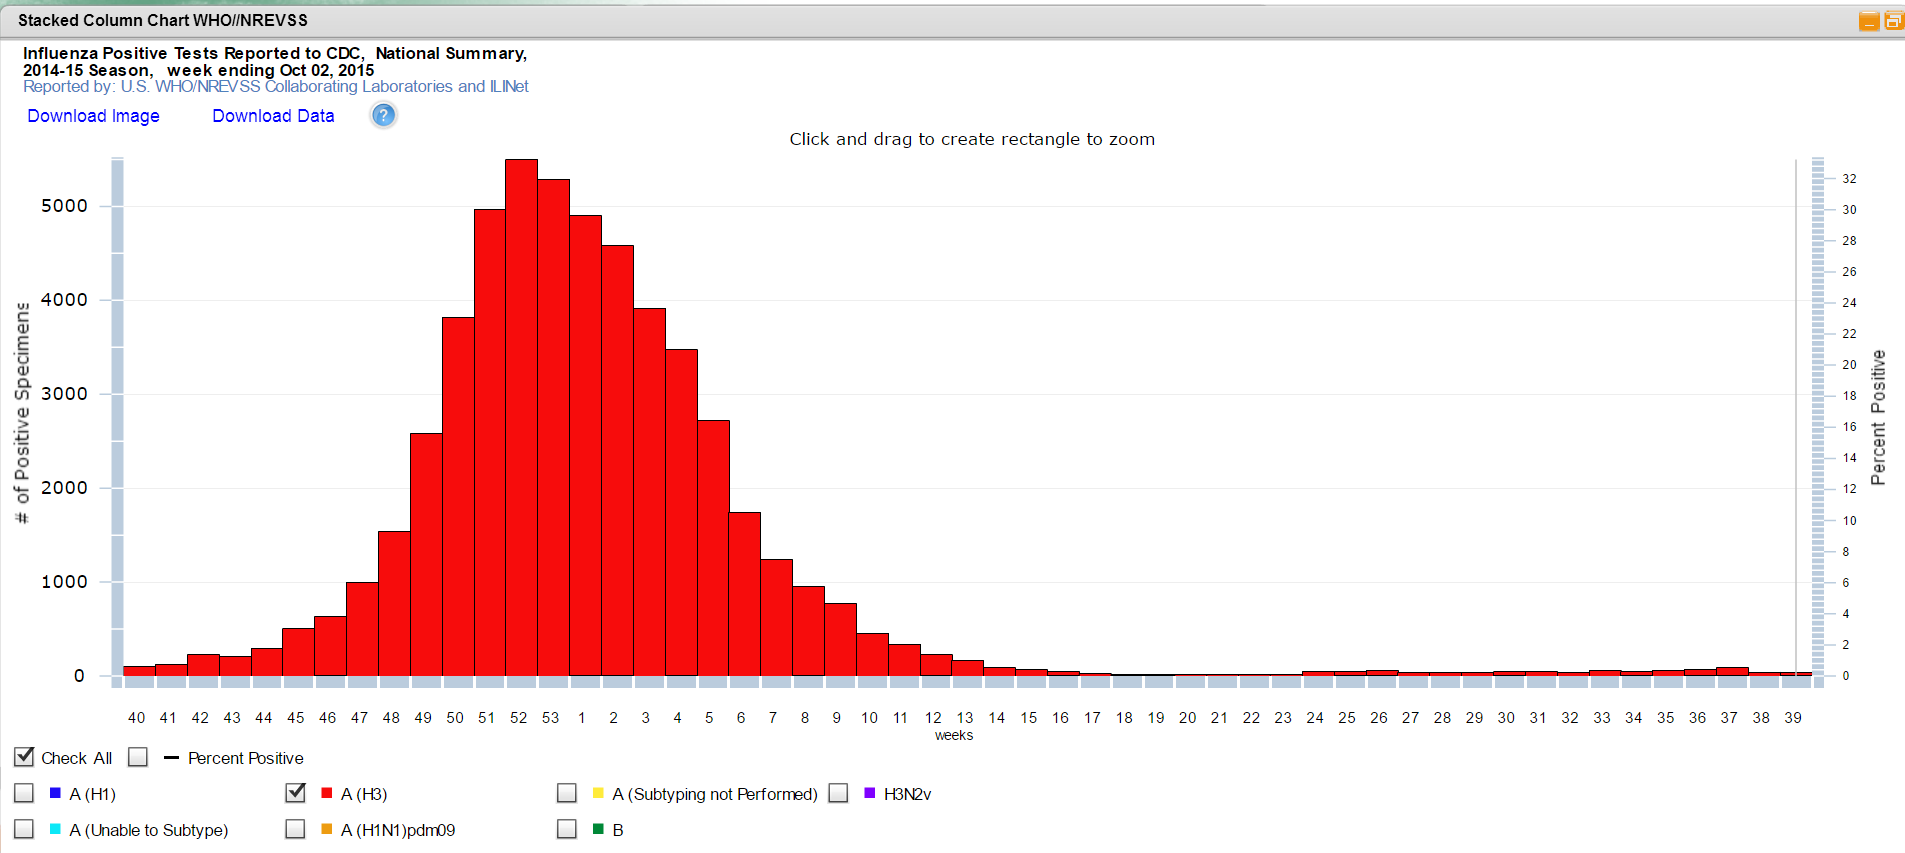
\includegraphics[height=5mm]{fig/H3} 
 U.S. WHO/NREVSS Collaborating Laboratories and ILNet.
 \href{http://gis.cdc.gov/grasp/fluview/fluportaldashboard.html}{`Stacked Column Chart WHO//NREVSS'} 
 Centers for Disease Control and Prevention.
 No longer available from \url{http://gis.cdc.gov/grasp/fluview/fluportaldashboard.html} (accessed 20 October 2015)}
}
\only<3|handout:0>{
\AnswerBar{3}{3}
\color{answercolor}\small

Let $t=0$ be the 40th week of 2014. Then we can model the spread of the virus like so:
\[P(t) = 100e^{kt}\]
We have one other data point:
$506=P(5)=100e^{5k}$, so we get
$e^k = 5.06^{1/5}$. Now our equation is:
\[P(t)=100(5.06)^{t/5}\]
We set it equal to 5000 and solve:
$5000=100(5.06)^{t/5}$ implies 
\[
(5.06)^{t/5}=50
\implies
\frac{t}{5}\log(5.06)=\log 50
\implies t=\frac{5\log 50}{\log(5.06)} \approx 12.06\]

Data from the CDC says Week 51 ($t=11$) had 4972
 cases, and 
Week 52 ($t=12$) had 5498
 cases.
\vfill
 
 Using the same formula, $10000=100(5.06)^{t/5}$ yields
 $t=\frac{5\log 100}{\log 5.06} \approx 14.2$ weeks; but the data shows that the flu season peaked with around 5,000 cases a week, and never got much higher.

}
\unote{Example~\eref{text}{eg:SDEpopgthA}}
\end{frame}
%----------------------------------------------------------------------------------------

%----------------------------------------------------------------------------------------
%----------------------------------------------------------------------------------------
\begin{frame}[t]
\begin{block}{Newton's Law of Cooling -- Equation~\eref{text}{eq:newtonCooling}}
The rate of change of temperature of an object is proportional to the difference in temperature between that object and its surroundings.



\pause
\[\frac{d\textcolor{C1}{T}}{dt}(t) = \textcolor{M4}{K}[\textcolor{C1}{T(t)}-\textcolor{M3}{A}]\]
where $\textcolor{C1}{T(t)}$ is the temperature of the object at time $t$, \textcolor{M3}{$A$} is the (constant) ambient temperature of the surroundings, and \textcolor{M4}{$K$} is some constant depending on the object.
\end{block}
\end{frame}
%----------------------------------------------------------------------------------------
%----------------------------------------------------------------------------------------
\begin{frame}[t]
\AnswerSpace\only<1>{\AnswerYes\QuestionBar{1}{6}}
\only<2>{\AnswerBar{1}{6}}
\[\frac{d\textcolor{C1}{T}}{dt}(t) = \textcolor{M4}{K}[\textcolor{C1}{T(t)}-\textcolor{M3}{A}]\]
$\textcolor{C1}{T(t)}$ is the temperature of the object, \textcolor{M3}{$A$} is the ambient temperature, \textcolor{M4}{$K$} is some constant.
\vfill
What is true of $K$?
\begin{enumerate}[A.]
\item $K\ge0$
\alert<2|handout:0>{\item $K\le0$}
\item $K=0$
\item $K$ could be positive, negative, or zero, depending on the object
\item I don't know
\end{enumerate}
\end{frame}
%----------------------------------------------------------------------------------------
%----------------------------------------------------------------------------------------
\begin{frame}[t]
\begin{block}{Newton's Law of Cooling -- Equation~\eref{text}{eq:newtonCooling}}
\[\frac{d\textcolor{C1}{T}}{dt}(t) = \textcolor{M4}{K}[\textcolor{C1}{T(t)}-\textcolor{M3}{A}]\]
$\textcolor{C1}{T(t)}$ is the temperature of the object, \textcolor{M3}{$A$} is the ambient temperature, and \textcolor{M4}{$K$} is some constant.
\end{block}

\[\textcolor{C1}{T(t)} = [\textcolor{C1}{T(0)}-\textcolor{M3}{A}]e^{\textcolor{M4}{K}t}+\textcolor{M3}{A}\]
is the only function satisfying Newton's Law of Cooling
\pause

\AnswerSpace\only<2,3>{\AnswerYes}
\only<2>{\QuestionBar{2}{6}}
\only<3>{\AnswerBar{2}{6}\QuestionBar{3}{6}}
\only<4->{\AnswerBar{3}{6}}

\begin{multicols}{2}
If $T(10)<A$, then:
\begin{itemize}
\item[A.] $K>0$
\item[B.]  $T(0)>0$
\item[C.]  $T(0)>A$
\alert<3-|handout:0>{\item[D.] $T(0)<A$}
\end{itemize}\columnbreak

\onslide<3->{
Evaluate $\displaystyle\lim_{t \rightarrow \infty} T(t)$.
\begin{itemize}
\alert<4-|handout:0>{\item[A.] $A$}
\item[B.] $0$
\item[C.]  $\infty$
\item[D.] $T(0)$
\end{itemize}
}

\end{multicols}

\end{frame}
%----------------------------------------------------------------------------------------

%----------------------------------------------------------------------------------------
%----------------------------------------------------------------------------------------
\begin{frame}
\QuestionBar{4}{6}\AnswerNo
What assumptions are we making that might not square with the real world?
\vfill

\begin{block}{Newton's Law of Cooling -- Equation~\eref{text}{eq:newtonCooling}}
\[\frac{d\textcolor{C1}{T}}{dt} = \textcolor{M4}{K}[\textcolor{C1}{T(t)}-\textcolor{M3}{A}]\]
$\textcolor{C1}{T(t)}$ is the temperature of the object, \textcolor{M3}{$A$} is the ambient temperature, and \textcolor{M4}{$K$} is some constant.
\end{block}


\begin{block}{Temperature of a Cooling Body -- Corollary~\eref{text}{cor:coolingDEsoln}}
\[\textcolor{C1}{T(t)} = [\textcolor{C1}{T(0)}-\textcolor{M3}{A}]e^{\textcolor{M4}{K}t}+\textcolor{M3}{A}\]
\end{block}



\end{frame}
%----------------------------------------------------------------------------------------
\begin{frame}[t]
\only<1-2>{\QuestionBar{5}{6}}
\note<1>{A farrier is a person who puts horseshoes on horses. They often double as blacksmiths, heating the shoes up in a forge and hitting them on an anvil to shape them. Then to cool the shoes down, they may dunk them in a bucket of water, like the photo.

We're making the very gross assumptions that the water stops boiling when the shoe hits 100 degrees, and the temperature of the river water is constant.}
\only<1>{\MoreSpace}
\only<1-2>{\AnswerYes
A farrier forms a horseshoe heated to $400^\circ$ C, then dunks it in a river at room-temperature ($25^\circ$ C). The water boils for 30 seconds. The horseshoe is safe for the horse when it's $40^\circ$ C. When can the farrier put on the horseshoe?

\only<1>{\vspace{-2mm}
\hfill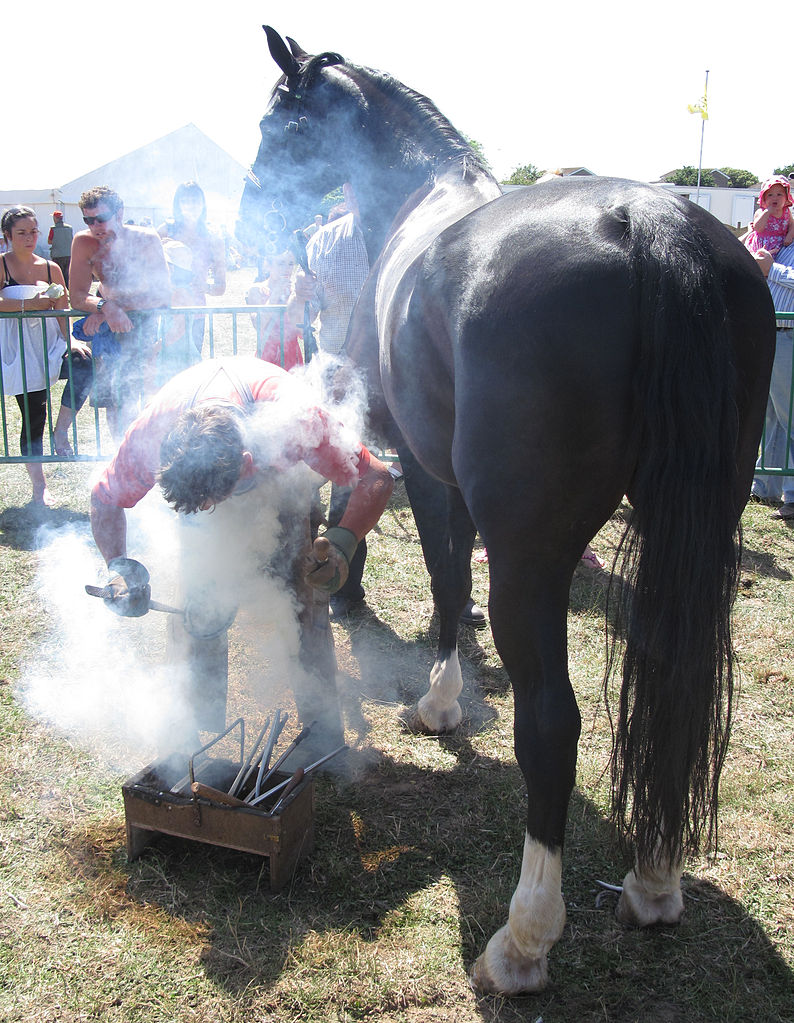
\includegraphics[scale=.4]{Clipart/farrier}}
\onslide<2>{\[T(t)=[T(0)-A]e^{Kt}+A\]}


\index{Public Domain by Man vyi via \url{https://commons.wikimedia.org/wiki/File:West_Show_Jersey_2010_farrier_f.jpg}, accessed October 2015}}

\only<3|handout:0>{
\AnswerBar{5}{6}
\color{answercolor}
We know: $T(0)=400$, $T(30)=100$, and $A=25$. We want to find $K$.
\begin{align*}
100=T(30) &= [T(0)-A]e^{30K}+A=375e^{30K}+25\\
\Rightarrow 75&=375e^{30K} \Rightarrow \frac{1}{5}=e^{30K} \Rightarrow K=\frac{-\log 5}{30}
\end{align*}
Now, we set $T(t)=40$ and solve for $t$:
\begin{align*}
40&=T(t)=375e^{\frac{-\log 5}{30}t}+25\\
15&=375e^{\frac{-log 5}{30}t}=375\cdot 5^{-t/30}\\
\frac{1}{25}&=5^{-t/30}\\
25&=5^{t/30}\\
2&=t/30
\end{align*}
So the farrier can put the shoe on after 60 seconds in the water.
}
\unote{Example~\eref{text}{eg:SDEcoolingA}}
\end{frame}
%----------------------------------------------------------------------------------------
%----------------------------------------------------------------------------------------
%----------------------------------------------------------------------------------------
%----------------------------------------------------------------------------------------
\begin{frame}[t]
\only<1>{
\QuestionBar{6}{6}
A glass of just-boiled tea is put on a porch outside. After ten minutes, the tea is $40^\circ$, and after 20 minutes, the tea is $25^\circ$. What is the temperature outside?
\note{This is a perennial frustration, but a good exercise. It anticipates a question in WeBWorK.}
\AnswerYes}
\only<2|handout:0>{\AnswerBar{6}{6}
\color{answercolor}
$T(0)=100$, so 
\begin{align*}
T(10)&=[100-A]e^{10K}+A= 100 e^{10K} +A\big(1-e^{10 K}\big)  = 40\\
T(20)&= [100-A]e^{20K}+A= 100 e^{20K} +A\big(1-e^{20 K}\big) =25
\end{align*} 
Solving both for $A$, we get
$A = \dfrac{40-100e^{10K}}{1-e^{10K}} = \dfrac{25-100e^{20K}}{1-e^{20K}}$
\vfill
Although this looks complicated, if we set $x=e^{10k}$, it simplifies to something we can easily solve.
}
\only<3|handout:0>{\AnswerBar{6}{6}
\color{answercolor}
\begin{align*}
A = \dfrac{40-100e^{10K}}{1-e^{10K}} &= \dfrac{25-100e^{20K}}{1-e^{20K}}\\
A = \dfrac{40-100x}{1-x} &= \dfrac{25-100x^2}{1-x^2}\\
(40-100x)(1-x^2)&=(25-100x^2)(1-x)\\
(40-100x)(1+x)(1-x)&=(25-100x^2)(1-x)\\
(40-100x)(1+x)&=25-100x^2\\
40-60x-100x^2&=25-100x^2\\
40-60x&=25\\
x=\frac{1}{4}\\
A = \dfrac{40-100x}{1-x} &=\dfrac{40-\frac{100}{4}}{1-\frac{1}{4}}=20
\end{align*}
It is 20 degrees outside.
}

\unote{Example~\eref{text}{eg:SDEcoolingB}}
\end{frame}
%----------------------------------------------------------------------------------------
%----------------------------------------------------------------------------------------
%----------------------------------------------------------------------------------------
%----------------------------------------------------------------------------------------

\note{Now a long list of questions, some of which you may have time for in class.}
%----------------------------------------------------------------------------------------
%----------------------------------------------------------------------------------------

\begin{frame}[t]
\only<1>{
\QuestionBar{1}{7}
In 1963, the US Fish and Wildlife Service recorded a bald eagle population of 487 breeding pairs. In 1993, that number was 4015. How many breeding pairs would you expect there were in 2006? What about 2015?
\vfill}
\only<2|handout:0>{
\QuestionBar{1}{7}
\centering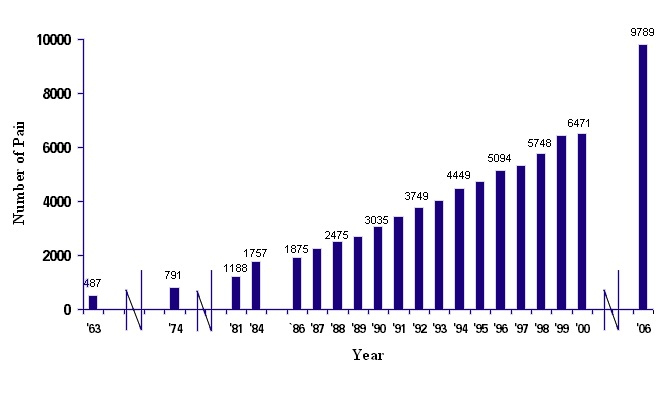
\includegraphics[width=\framewidth]{fig/eaglechart}
\index{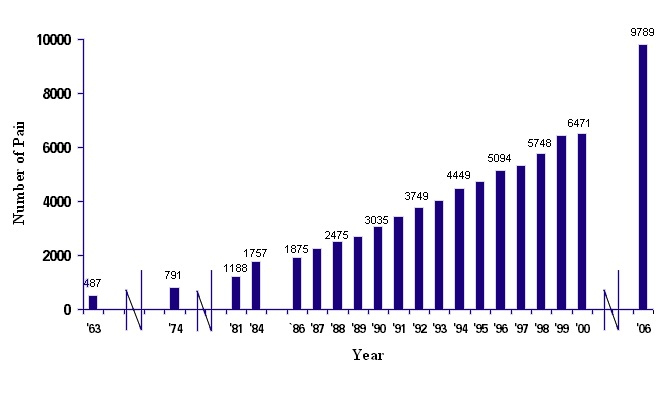
\includegraphics[height=5mm]{fig/eaglechart} 
\href{http://www.fws.gov/midwest/eagle/population/chtofprs.html}{`Chart of Bald Eagle Breeding Pairs in Lower 48 States'}.  Eagle nesting data, US Fish and Wildlife Service Midwest Region (accessed 19 October 2016)}
}
\only<3|handout:0>{
\AnswerBar{1}{7}
\small
\color{answercolor}
Since we don't have a better model, let's assume the population $P$ of nesting pairs follows:
\[P(t) = P(0)e^{Kt}\]
for some constant $K$. 

\medskip
To fit the data we have, let $t=0$ represent 1963, so $P(0)=487$. Then \[4015=P(30)=487e^{30K}\]
 so $e^K=\left(\frac{4015}{487} \right)^{1/30}$.

\medskip
 Now we use this to predict $P(43)$ (since 2006 is 43 years after 1963) and $P(52)$ (since 2015 is 52 years after 1963).
\[
P(43) = 487(e^K)^{43} = 487\left( \frac{4015}{487}\right)^{43/30} \approx 10 016
\]

So we guess in 2016 there were about 10,016 breeding pairs in the lower 48.

\[ P(52) = 487(e^K)^{52} = 487\left( \frac{4015}{487}\right)^{52/30} 
   \approx 18 860\]
}
\end{frame}
%----------------------------------------------------------------------------------------
%----------------------------------------------------------------------------------------
%----------------------------------------------------------------------------------------
\begin{frame}[t]\AnswerSpace
\only<1>{\QuestionBar{2}{7}\AnswerYes}
\only<2>{\AnswerBar{2}{7}}
\note<1>{Wood bison were thought to be extinct, except for populations that had interbred with plains bison. A pure-blooded population was discovered in Canada and bred in captivity to increase their numbers. Later, Canada sent some of these descendants to Alaska, where the Alaska Wildlife Conservation Center cared for them and increased their numbers, eventually releasing some. After being extinct in Alaska for around a century, there are once again wood bison in the wild.}
\note<2>{It can often seem like scientists have unknowable algorithms behind their predictions. When we understand where a model comes from, we can better understand its limitations. For example, the model we (and ADF\&G) are using is simply that bison will reproduce in proportion to their population. It's useful to think about when that assumption might not hold.}
\href{http://www.adfg.alaska.gov/static/species/speciesinfo/woodbison/pdfs/er_no_appendices.pdf}{
link: Wood Bison Restoration in Alaska, Alaska Department of Fish and Game}\vfill
Excerpt:
\begin{quote}
Based on experience with reintroduced populations elsewhere, wood bison would be expected to increase at a rate of 15\%-25\% annually after becoming established.... With an average annual growth rate of 20\%, an initial precalving population of 50 bison would increase to 500 in approximately 13 years.
\end{quote}
\vfill
\NowYou Are they using our same model? 
\vfill\pause\color{answercolor}
\answer{Our model gives the same result.}

\index{Alaska Department of Fish and Game, Division of Wildlife Conservation. (April 2007). Wood Bison Restoration in Alaska: A Review of Environmental and Regulatory Issues and  Proposed Decisions for Project Implementation,  p. 11. \url{http://www.adfg.alaska.gov/static/species/speciesinfo/woodbison/pdfs/er_no_appendices.pdf} (accessed 2015 or 2016)}
\end{frame}
%----------------------------------------------------------------------------------------
%\begin{frame}
%http://www.wildlifecollisions.ca/docs/nahanniherdstatus2007.pdf
%p15 growth rate
%
%\url{http://www.enr.gov.nt.ca/sites/default/files/strategies/wood_bison_management_strategy.pdf}
%NWT populations
%\end{frame}
%----------------------------------------------------------------------------------------
%----------------------------------------------------------------------------------------
\begin{frame}[t]{Compound Interest}
\AnswerSpace\only<1-2>{\AnswerYes\QuestionBar{3}{7}}
\only<3->{\AnswerBar{3}{7}}
\note<1>{Probably students have seen a derivation of the compound interest formula that didn't use DE. Since the balance grows proportionally to how much is in it, it system satisfies the same DE, so it'll have the same solution.}
Suppose you invest \$10,000 in an account that accrues interest each month. After one month, your balance (with interest) is \$10,100. How much money will be in your account after a year?\pause\vfill\color{answercolor}

Compound interest is calculated according to the formula $Pe^{rt}$, where $r$ is the interest rate and $t$ is time.\pause\vfill

\small
\answer{\abovedisplayskip=0pt
Measuring time in months,
\begin{align*}
10000e^{r \cdot 1} &= 10100\\
e^r&=\frac{10100}{10000}=1.01\\
10000e^{12r}&=10000\cdot(e^r)^{12}=10000\cdot 1.01^{12} \approx11268.25
\end{align*}}
\end{frame}

%----------------------------------------------------------------------------------------
\begin{frame}[t]{Carrying Capacity}
\only<1>{\QuestionBar{4}{7}\AnswerYes}
\only<2>{\AnswerBar{4}{7}}
For a population of size $P$ with unrestricted access to resources, let $\beta$ be the average number of offspring each breeding pair produces per generation, where a generation has length $t_g$. Then \alert<3>{$b=\frac{\beta-2}{2t_g}$ is the net birthrate (births minus deaths) per member per unit time}. This yields \alert<1>{$\frac{dP}{dt}(t) = bP(t)$}, hence:\pause
\answer{\[P(t)=P(0)e^{bt}\]}
\vfill\pause

But as resources grow scarce, $b$ might change.

\end{frame}

%----------------------------------------------------------------------------------------
\begin{frame}[t]{Carrying Capacity}\AnswerSpace
$b$  is the net birthrate (births minus deaths) per member per unit time. 
If $K$ is the carrying capacity of an ecosystem, we can model $b=b_0(1-\frac{P}{K})$. 

\begin{tikzpicture}
\myaxis{P}{0}{8}{b}{1}{1}
\xcoord{4}{K}
\draw[thick,C1] plot[domain=0.2:8](\x,{1-\x/4});
\end{tikzpicture}\pause

\NowYou Describe to your neighbour what the following mean in terms of the model:
\begin{itemize}
\item $b>0$, $b=0$, $b<0$
\item $P=0$, $P>0$, $P<0$
\end{itemize}
\only<2->{\AnswerNo\QuestionBar{5}{7}}
\end{frame}

%----------------------------------------------------------------------------------------
\begin{frame}[t]{Carrying Capacity}

Then:
\[\frac{dP}{dt}(t) =\underbrace{ b_0\left(1-\frac{P(t)}{K}\right)}_{\text{per capita birthrate}}P(t)\]
\pause

This is an example of a differential equation that we don't have the tools to solve. (If you take more calculus, though, you'll learn how!)

It's also an example of a way you might tweak a model so its assumptions better fit what you observe.
\end{frame}

%----------------------------------------------------------------------------------------
\begin{frame}[t]{Radiocarbon Dating}
\unote{Example~\eref{text}{eg:carbonDating}}
\note<1>{Read the question first. Note that we can do this two ways: there's an easy approximation in your head, and a pen-and-paper calculation. First, do the rough approximation.}
\only<1-2>{\AnswerSpace\only<2>{\AnswerYes}
\only<2>{\QuestionBar{6}{7}}\only<3>{\AnswerBar{6}{7}}
Researchers at Charlie Lake in BC have found evidence\only<1>{\footnote{ \url{http://pubs.aina.ucalgary.ca/arctic/Arctic49-3-265.pdf}}} of habitation dating back to around 8500 BCE. For instance, a butchered bison bone was radiocarbon dated to about 10,500 years ago.\vfill

Suppose a comparable bone of a bison alive today contains 1$\mu$g of $^{14}C$. If the half-life of $^{14}C$ is about 5730 years, roughly how much $^{14}C$ do you think the researchers found in the sample?\vfill
\pause

\onslide<2->{
\begin{multicols}{2}\begin{itemize}
\item[A.] About $\frac{1}{10,500}$ $\mu$g
\alert<3-|handout:0>{\item[B.] About $\frac{1}{4}$ $\mu$g}
\item[C.] About $\frac{1}{2}$ $\mu$g
\item[D.] About 1 $\mu$g
\item[E.] I'm not sure how to estimate this
\end{itemize}\end{multicols}}

\index{Driver et.al. Stratigraphy, Radiocarbon Dating, and Culture History of Charlie Lake Cave, British Columbia. \textit{ARCTICVOL. 49, no. 3 (September 1996) pp. 265 – 277}. \url{http://pubs.aina.ucalgary.ca/arctic/Arctic49-3-265.pdf} (accessed 2015 or 2016)}
}
\only<3|handout:0>{
\AnswerBar{6}{7}
\color{answercolor}First, an estimate; 10500 is not so far off from 2(5730),
i.e. two half-lives, so we might guess that there is roughly a $(\frac{1}{2})^2=\frac{1}{4}$ of  a microgram left.\vfill\pause
\note<1>{If we wanted to calculate more precisely....}
We know $Q(t)=Ce^{-kt}=e^{-kt}$ $\mu$g. We want to find $Q(10500)$, so we need to solve for $k$. Since we know the half-life: to do this, solve \[\frac{1}{2}=e^{-k\cdot 5730}\quad\text{to get}\quad k=\frac{\log 2}{5730}\] 
Now:
\[
Q(10500)=e^{-\frac{\log 2}{5730}\cdot 10500} = 2^{-\frac{10500}{5730}} 
        \approx 0.28\ \mu\text{g}
\]
}
\end{frame}
%----------------------------------------------------------------------------------------
%----------------------------------------------------------------------------------------
%----------------------------------------------------------------------------------------
\begin{frame}[t]
\only<1>{
Suppose a body is discovered at 3:45 pm, in a room held at $20^\circ$, and the body's temperature is $27^\circ$, not the normal $37^\circ$. At 5:45 pm, the temperature of the body has dropped to $25.3^\circ$. When did the inhabitant of the body die?\vfill
\AnswerYes\QuestionBar{7}{7}
}
\color{answercolor}\small
\only<2|handout:0>{\AnswerBar{7}{7}
Set our time so that $t=0$ is 3:45pm and $t=2$ is 5:45pm. Then
$T(0)=27$, $T(2)=25.4$, and $A=20$ . Now:
\[T(t)=[27-20]e^{Kt}+20=7e^{Kt}+20\]
Using what we know about 5:45pm:
\[
7e^{2K}+20=T(2)=25.3
\]
so 
\[
7e^{2K}=5.3 
\implies e^{2K}=\frac{5.3}{7}
\implies e^K=\left(\frac{5.3}{7}\right)^{1/2}
\]

Now:
\[T(t)=7e^{Kt}+20=7\left(\frac{5.3}{7}\right)^{t/2}+20\]
So we set $T(t)=37$ and solve for $t$.}

\only<3|handout:0>{\AnswerBar{7}{7}
\begin{align*}
7\left(\frac{5.3}{7}\right)^{t/2}+20&=37\\
7\left(\frac{5.3}{7}\right)^{t/2}&=17\\
\left(\frac{5.3}{7}\right)^{t/2}&=\frac{17}{7}\\
\frac{t}{2}&%=\log_{\frac{5.3}{7}}\left(\frac{17}{7} \right) 
           = \dfrac{\log (17/7)}{\log (5.3/7)}\\
t&=2\dfrac{\log (17/7)}{\log(5.3/7)} \approx -6.4\end{align*}

So the person died about 6.4 hours before 3:45pm. 
Now 0.4 hours is 24 minutes.
So 6 hours and 24 minutes before 3:45 pm is 6 hours before 3:21pm, which is 9:21 am.}
\unote{Example~\eref{text}{eg:SDEcoolingC}}
\end{frame}
%----------------------------------------------------------------------------------------
%----------------------------------------------------------------------------------------

%----------------------------------------------------------------------------------------
%----------------------------------------------------------------------------------------
%\begin{frame}[t]
%In the peer-reviewed journal Eurosurveillace, Volume 19, Issue 36, 11 Sept 2014, there is an article titled EARLY TRANSMISSION DYNAMICS OF EBOLA VIRUS DISEASE (EVT), WEST AFRICA, MARCH TO AUGUST 2014. Authors H Nishiura and G Chowell try to determine how fast the current Ebola outbreak is spreading.
%\begin{enumerate}[label=(\alph*)]
%\item Suppose a disease spreads as follows: Every person with the disease gives it to two healthy people. It takes one day for this to happen, and after that day, the original person is not contagious. Suppose we start with one sick person on day 1. How many people get sick on day $n$?
%\item On Sept 14, Wired.com published an article by Maryn McKenna titled
%The Mathematics of Ebola Trigger Stark Warnings: Act Now or Regret It (available on the web at http://www.wired.com/2014/09/r0-ebola). In it, McKenna wrote the following:
%\begin{quote}
%The most arresting is a piece published last week in the journal Eurosurveillance, which is the peer-reviewed publication of the European Centre for Disease Prevention and Control (the EU’s Stockholm-based version of the US CDC). The piece is an attempt to assess mathematically how the epidemic is growing, by using case reports to determine the “reproductive number.” (Note for non-epidemiology geeks: The basic reproductive number — usually shorted to R0 or “R-nought” — expresses how many cases of disease are likely to be caused by any one infected person. An R0 of less than 1 means an outbreak will die out; an R0 of more than 1 means an outbreak can be expected to increase. If you saw the movie Contagion, this is what Kate Winslet stood up and wrote on a whiteboard early in the film.)
%
%The Eurosurveillance paper, by two researchers from the University of Tokyo and Arizona State University, attempts to derive what the reproductive rate has been in Guinea, Liberia and Sierra Leone. (Note for actual epidemiology geeks: The calculation is for the effective reproductive number, pegged to a point in time, hence actually Rt.) They come up with an R of at least 1, and in some cases 2; that is, at certain points, sick persons have caused disease in two others.
%\end{quote}
%Explain the sentence:  ``An R0 of less than 1 means an outbreak will die out; an R0 of more than 1 means an outbreak can be expected to increase.'' in terms of what you've learned in this class.
%\item In the Nishura-Chowell paper, the abstract reads as follows:
%\begin{quote}
%The effective reproduction number, $R_t$, of Ebola virus disease was estimated using country-specific data reported from Guinea, Liberia and Sierra Leone to the World Health Organization from March to August, 2014. Rt for the three countries lies consistently above 1.0 since June 2014. Country-specific $R_t$ for Liberia and Sierra Leone have lied between 1.0 and 2.0. $R_t<2$ indicate that control could be attained by preventing over half of the secondary transmissions per primary case.
%\end{quote}
%Discuss this quote, in the context of geometric sequences. In particular: why would ``preventing over half'' control the outbreak? What must they mean by ``control?''
% \item On the next page is the graph from the Nishura-Chowell paper. How do you think they determined the value of R0?
% Do you think this outbreak fits the standard geometric model?
%% \begin{landscape}
%% \includegraphics[scale=0.5]{Nishiura_fig1.jpg}
%% \end{landscape}
%\end{enumerate}
%\end{frame}
%----------------------------------------------------------------------------------------
%----------------------------------------------------------------------------------------
%----------------------------------------------------------------------------------------
%----------------------------------------------------------------------------------------
%----------------------------------------------------------------------------------------
%----------------------------------------------------------------------------------------
%----------------------------------------------------------------------------------------
%----------------------------------------------------------------------------------------
%----------------------------------------------------------------------------------------
%----------------------------------------------------------------------------------------